% D1 - System context. Who the system serves, and what crosses its boundary.
%
% Deliberately the only diagram with no technology on it: the point of a context
% diagram is that a reader who knows nothing about Kafka can still see what the
% system is for and who depends on it.
\documentclass[border=8pt]{standalone}
% Shared styling for every report diagram.
%
% One colour convention across all four, stated in the legend on D2:
%   BLUE   speed path    - the approximate, low-latency half
%   GREEN  batch path    - the exact, recomputed half
%   GREY   infrastructure- stores and brokers that belong to neither path
%   ORANGE serving       - where the two are reconciled
%
% TikZ rather than draw.io: the report is LaTeX, so these compile as vector art with
% no external asset pipeline, the source is version-controlled beside the code, and
% fonts match the body text exactly. A diagram that can be regenerated from source is
% also a diagram that cannot silently drift from the system it describes.

\usepackage{tikz}
\usepackage{xcolor}
\usetikzlibrary{positioning,arrows.meta,fit,backgrounds,calc,shapes.geometric}

\definecolor{speedblue}{HTML}{1F6FB2}
\definecolor{speedbg}{HTML}{E3F0FA}
\definecolor{batchgreen}{HTML}{2E7D4A}
\definecolor{batchbg}{HTML}{E4F3E8}
\definecolor{servorange}{HTML}{C2660A}
\definecolor{servbg}{HTML}{FCEDDD}
\definecolor{infragrey}{HTML}{5A6672}
\definecolor{infrabg}{HTML}{ECEFF1}
\definecolor{edgegrey}{HTML}{444C54}

\tikzset{
  box/.style={
    draw, rounded corners=2pt, align=center, inner sep=5pt,
    font=\scriptsize, minimum height=8mm, line width=0.5pt,
  },
  speed/.style ={box, draw=speedblue,  fill=speedbg,  text=black},
  batch/.style ={box, draw=batchgreen, fill=batchbg,  text=black},
  serv/.style  ={box, draw=servorange, fill=servbg,   text=black},
  infra/.style ={box, draw=infragrey,  fill=infrabg,  text=black},
  ext/.style   ={box, draw=edgegrey, fill=white, dashed, text=black},
  flow/.style  ={-{Stealth[length=4pt]}, draw=edgegrey, line width=0.5pt},
  speedflow/.style={flow, draw=speedblue},
  batchflow/.style={flow, draw=batchgreen},
  lbl/.style   ={font=\tiny\itshape, text=edgegrey, inner sep=1.5pt},
  zone/.style  ={draw=edgegrey, dashed, rounded corners=3pt, line width=0.4pt,
                 inner sep=7pt},
  % fill=white matters: these labels sit ON the dashed zone border, and without
  % an opaque background the border line runs straight through the text and
  % reads as a strike-through.
  ztitle/.style={font=\scriptsize\bfseries, text=edgegrey, fill=white,
                 inner xsep=3pt, inner ysep=1pt},
}

\begin{document}
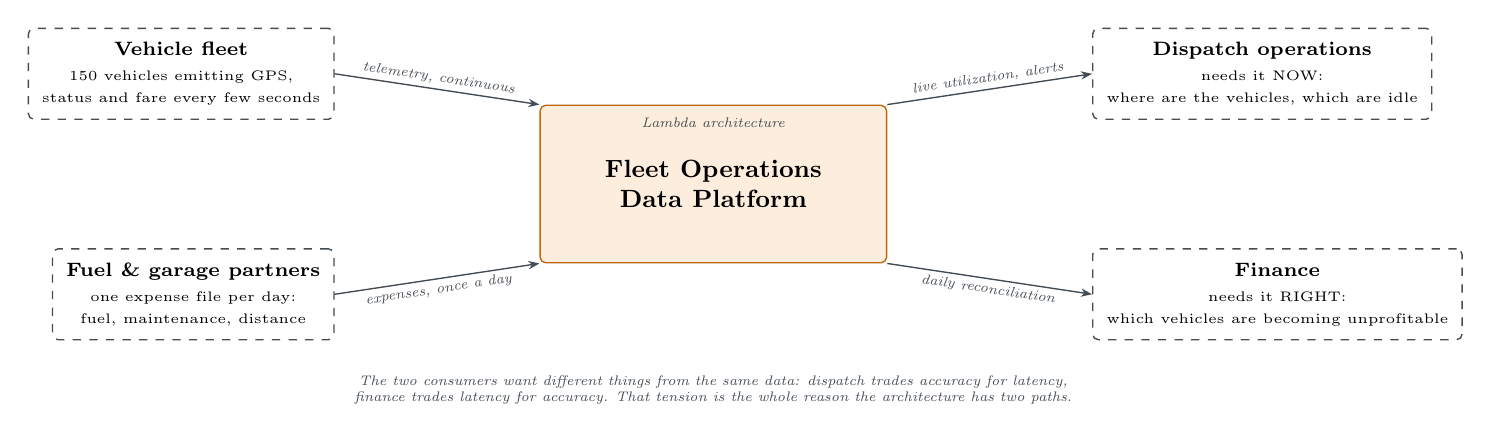
\begin{tikzpicture}[node distance=9mm]

\node[box, draw=servorange, fill=servbg, minimum width=44mm, minimum height=20mm,
      font=\small\bfseries] (sys)
  {Fleet Operations\\Data Platform};
\node[font=\tiny\itshape, text=edgegrey, below=0.5mm of sys.north, anchor=north]
  {Lambda architecture};

% ---------------------------------------------------------------- actors in
\node[ext, left=26mm of sys, yshift=14mm, minimum width=30mm] (drivers)
  {\textbf{Vehicle fleet}\\[1pt]\tiny 150 vehicles emitting GPS,\\\tiny status and fare
   every few seconds};
\node[ext, left=26mm of sys, yshift=-14mm, minimum width=30mm] (partners)
  {\textbf{Fuel \& garage partners}\\[1pt]\tiny one expense file per day:\\\tiny fuel,
   maintenance, distance};

% ---------------------------------------------------------------- actors out
\node[ext, right=26mm of sys, yshift=14mm, minimum width=30mm] (dispatch)
  {\textbf{Dispatch operations}\\[1pt]\tiny needs it NOW:\\\tiny where are the vehicles,
   which are idle};
\node[ext, right=26mm of sys, yshift=-14mm, minimum width=30mm] (finance)
  {\textbf{Finance}\\[1pt]\tiny needs it RIGHT:\\\tiny which vehicles are becoming
   unprofitable};

% ---------------------------------------------------------------- edges
\draw[flow] (drivers.east)  -- node[lbl, above, sloped] {telemetry, continuous} (sys.north west);
\draw[flow] (partners.east) -- node[lbl, below, sloped] {expenses, once a day} (sys.south west);
\draw[flow] (sys.north east) -- node[lbl, above, sloped] {live utilization, alerts} (dispatch.west);
\draw[flow] (sys.south east) -- node[lbl, below, sloped] {daily reconciliation} (finance.west);

% ---------------------------------------------------------------- the tension
\node[font=\tiny\itshape, text=edgegrey, align=center, below=13mm of sys]
  {The two consumers want different things from the same data: dispatch trades accuracy
   for latency,\\ finance trades latency for accuracy. That tension is the whole reason
   the architecture has two paths.};

\end{tikzpicture}
\end{document}
